% Drawing 152/01-5 -- folder 152, batch 01, archive page 3 (PDF page 4).
% Transcription: bas du feuillet, trois figures au crayon : à gauche un arc épais portant trois points marqués, d'où partent vers l'intérieur un trait, une bosse et un second trait ; au milieu un grand cercle pâle, avec en bas une petite bosse et quelques points marqués ; à droite un petit cercle d'où rayonnent quatre traits, relié vers la gauche par l'un d'eux.
% Kind: arc with chords, a large faint circle, a small radiating circle. Method 2 (schematic redraw from the facsimile). Status: partial.
% Notes: Left: the heavy arc with three marked points on it, a stroke going down from it at the left, a bump (a small chord) in the middle and a second stroke going down at the right. Middle: the large faint circle (an ellipse fitted to it), with a small bump and five marked points at its bottom. Right: the small circle with three marks on it and four strokes radiating from it (two up, one to the lower right, one long to the lower left, towards the large circle, which it does not reach). Still differs: positions read off a wide crop; the large circle is drawn once (he went round it twice). This is the pair « deux disques reliés par une arête, le second plus petit et rayonnant » of the note of the transcription, if the long stroke of the small circle is taken as the edge. Redrawn 2026-11-12 (issue 128): to check again.
% Coordinates: 1 unit = 1 mm = 1/100 of the crop width (bbox in page fractions: [0.15, 0.66, 0.92, 0.84]).
% Redrawn by Claude (claude-fable-5-2), issue #128, 2026-11-12; not checked by a human; not compiled (no TeX in the session).
% Rights: reproduces part of the work -- behind RENDER_TRANSCRIPTS, never published by itself.
\documentclass[tikz,border=3pt]{standalone}
\usepackage{amsmath,amssymb}
\usetikzlibrary{patterns,arrows.meta}
\tikzset{pencil/.style={black!45}, struck/.style={black!35}, mpt/.style={circle,draw,inner sep=1.3pt}, pt/.style={circle,fill,inner sep=0.9pt}, opt/.style={circle,draw,fill=white,inner sep=1.1pt}}
\begin{document}
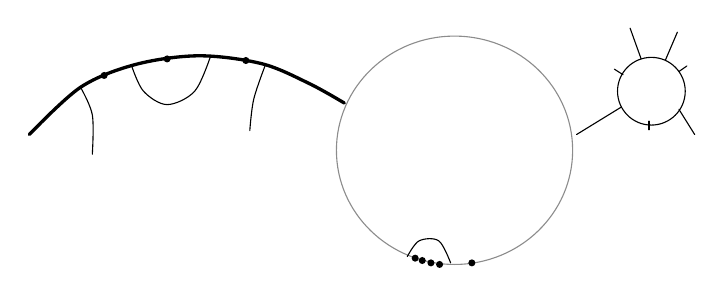
\begin{tikzpicture}[x=1mm,y=1mm,line cap=round,line join=round,font=\scriptsize]
\draw[very thick] plot[smooth, tension=0.55] coordinates {(6.5,-14.5) (13,-8.5) (20,-5.6) (28,-4.5) (36,-5.5) (42,-8) (46.5,-10.5)};
\node[pt] at (16,-7) {};
\node[pt] at (24,-4.9) {};
\node[pt] at (34,-5.1) {};
\draw plot[smooth, tension=0.55] coordinates {(13,-8.5) (14.5,-12) (14.5,-17)};
\draw plot[smooth, tension=0.55] coordinates {(19.5,-5.8) (21,-9) (24,-10.7) (27.5,-9) (29.5,-4.6)};
\draw plot[smooth, tension=0.55] coordinates {(36.5,-5.6) (35,-10) (34.5,-14)};
\draw[pencil] (60.5,-16.5) ellipse[x radius=15, y radius=14.5];
\draw plot[smooth, tension=0.55] coordinates {(54.5,-30) (56,-28) (58.5,-28) (60,-30.8)};
\node[pt] at (55.5,-30.2) {};
\node[pt] at (56.4,-30.5) {};
\node[pt] at (57.5,-30.8) {};
\node[pt] at (58.6,-31) {};
\node[pt] at (62.7,-30.8) {};
\draw (85.5,-9) circle[radius=4.3];
\draw (82.8,-1) -- (84.2,-4.9);
\draw (88.8,-1.5) -- (87.3,-5);
\draw (76,-14.5) -- (81.7,-11);
\draw (89,-11.3) -- (91,-14.5);
\draw (80.8,-6.2) -- (81.9,-6.9);
\draw (89,-6.5) -- (90,-5.8);
\draw (85.2,-12.8) -- (85.2,-13.9);
\end{tikzpicture}
\end{document}
